\documentclass[12pt,letterpaper]{exam}
\usepackage[lmargin=1in,rmargin=1in,tmargin=1in,bmargin=1in]{geometry}
\usepackage{../style/exams}

% -------------------
% Course & Exam Information
% -------------------
\newcommand{\course}{MAT 308: Exam 3}
\renewcommand{\term}{Fall -- 2023}
\newcommand{\examdate}{12/14/2023}
\newcommand{\timelimit}{`$\infty$' Minutes}

\setbool{hideans}{true} % Student: True; Instructor: False


% -------------------
% Content
% -------------------
\begin{document}

\examtitle
\instructions{Write your name on the appropriate line on the exam cover sheet. This exam contains \numpages\ pages (including this cover page) and \numquestions\ questions. Check that you have every page of the exam. Answer the questions in the spaces provided on the question sheets. Be sure to answer every part of each question and show all your work. If you run out of room for an answer, continue on the back of the page --- being sure to indicate the problem number.} 
\scores
\bottomline
\newpage

% ---------
% Questions
% ---------
\begin{questions}

% Question 1
\newpage
\question[10] There have been numerous studies showing that physicians, medical staff, and patients have trouble understanding and interpreting conditional probabilities. One study showed that physicians had serious misunderstandings about the following hypothetical statistics problem: the probability of breast cancer is 2\% for women of a particular age group participating in a routine screening. The medical procedure used to identify this breast cancer is 97\% accurate at identifying cancer when it is present and misidentifies a woman as having breast cancer when do not 2\% of the time.
	\begin{enumerate}[(a)]
	\item Find the probability that a woman in this age group will test positive for breast cancer. 
	\item Find the probability that a woman in this age group will test positive for breast cancer or have breast cancer. 
	\item Find the probability that a woman in this age group will have breast cancer and test positive.
	\item If a woman in this age group tests positive for breast cancer, what is the probability that she actually has cancer? 
	\end{enumerate}



\newpage



% Question 2
\newpage
\question[10] Showing all your work and fully justifying your reasoning, respond to the following:
	\begin{enumerate}[(a)]
	\item Is the graph shown below a tree? Explain.
		\begin{figure}[h]
		\centering
		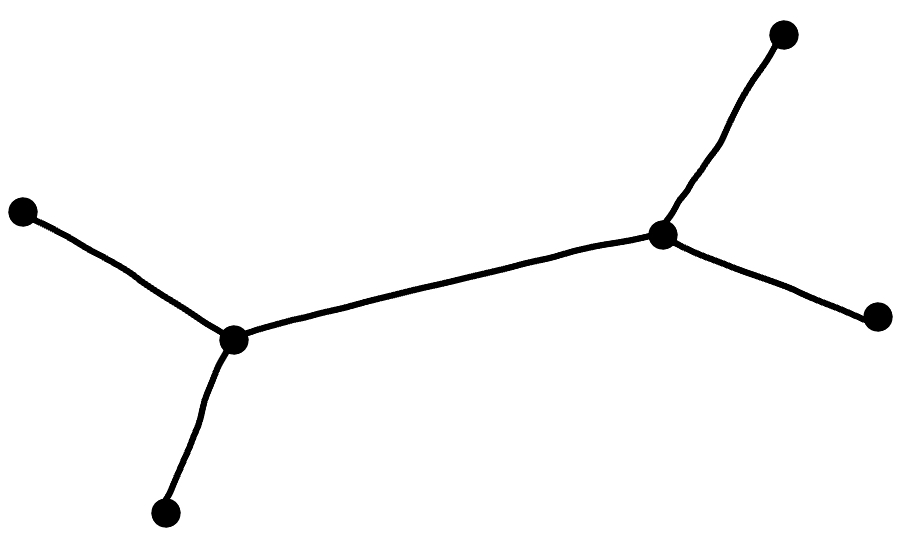
\includegraphics[width=0.15\textwidth]{graph1.jpg}
		\end{figure}
	
	\item What is the degree of a tree with $n$ vertices? 
	\item Are all trees with the same number of vertices isomorphic? If so, explain why. If not, give a counterexample. 
	\item Are there always unique paths between distinct vertices in a tree with $n \geq 1$ vertices? If so, explain why. If not, give a counterexample. 
	\end{enumerate}



\newpage



% Question 3
\newpage
\question[10] Define a \textit{pseudo tripartite} graph on $(m, n, p)$ vertices, denoted $K_{m, n, p}$, as follows:
	\begin{enumerate}[(i)]
	\item $K_{m,n,p}$ has vertices $v_1, v_2, \ldots, v_m$, $w_1, w_2, \ldots, w_n$, and $x_1, x_2, \ldots, x_p$.
	\item There exists a unique edge connecting $v_i$ and $w_j$ for all $i= 1, \ldots, m$ and $j= 1, \ldots, n$ and there exists a unique edge connecting $w_r$ and $x_s$ for all $r= 1, \ldots, n$ and $s= 1, \ldots, p$. 
	\item There exists no edge between $v_i$ and $v_j$ for all $i, j$. There exists no edge between $w_i$ and $w_j$ for all $i, j$. There exists no edge between $x_i$ and $x_j$ for all $i, j$. 
	\end{enumerate}

Given the definition above, complete the following:
\begin{enumerate}[(a)]
\item Sketch $K_{3, 2, 4}$.
\item What is $|V(K_{m, n, p})|$? Explain. 
\item What is $|E(K_{m, n, p})|$? Explain. 
\item Is $K_{m, n, p}$ connected? Explain. 
\item Can $K_{m, n, p}$ be isomorphic to $K_{r, s}$ for any $m, n, p, r, s \geq 1$? Explain. 
\end{enumerate}



\newpage



% Question 4
\newpage
\question[10] Let $G$ be the graph whose adjacency matrix, $A_G$, is given below.
	\[
	\begin{pmatrix}
	1 & 1 & 0 & 1 \\
	0 & 0 & 1 & 0 \\
	1 & 0 & 0 & 0 \\
	0 & 0 & 1 & 0 
	\end{pmatrix}
	\]

\begin{enumerate}[(a)]
\item Sketch $G$. 
\item If $G'$ has adjacency matrix $A_{G'}$ and $A_G= A_{G'}$, must it be that $G$ and $G'$ are isomorphic? 
\item Can $G$ be isomorphic to the graph below? Explain. 
	\begin{figure}[h]
	\centering
	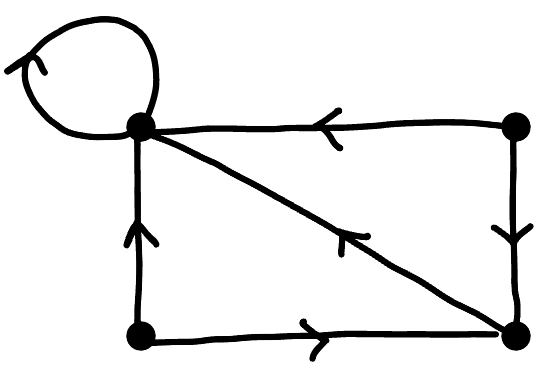
\includegraphics[width=0.18\textwidth]{graph2.jpg}
	\end{figure}
\end{enumerate}



\newpage



% Question 5
\newpage
\question[10] Consider the floor plan shown below.
	\begin{figure}[h]
	\centering
	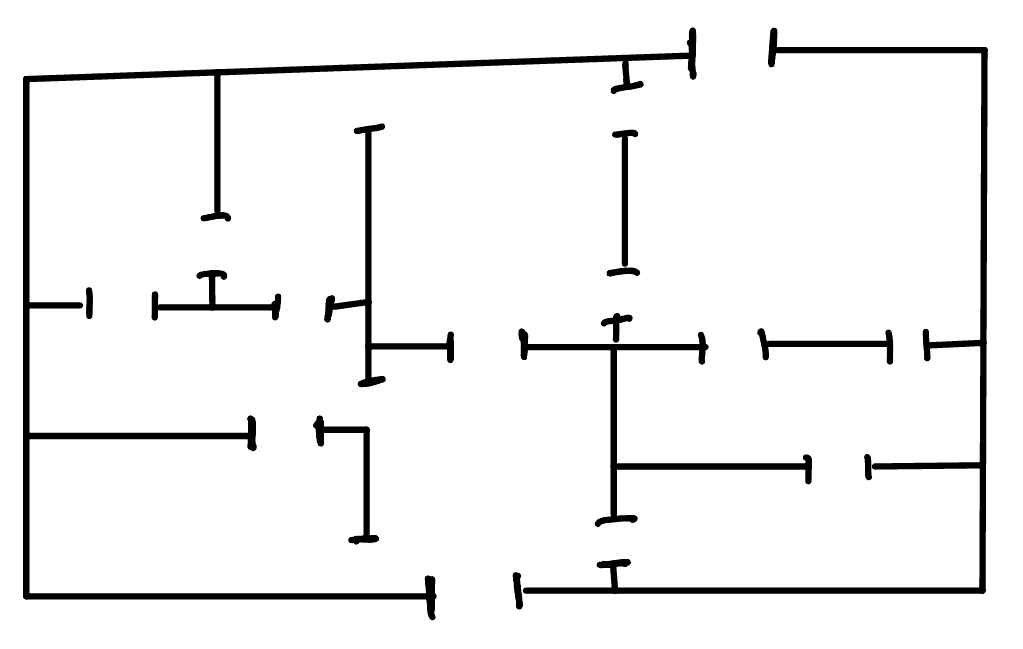
\includegraphics[width=0.3\textwidth]{graph3.jpg}
	\end{figure}

\begin{enumerate}[(a)]
\item Is it possible to start at the front door and walk through each door of the house once and end at the back door? Explain. 
\item Is it possible to find a `path' that starts and ends in the same room such that you walk through each room in the house once? Explain. 
\item Is it possible to find a `path' that starts and ends in the same room such that you walk through each door in the house once? Explain. 
\end{enumerate}



\newpage



% Question 6
\newpage
\question[10] Consider the graph $G$ show below.
	\begin{figure}[h]
	\centering
	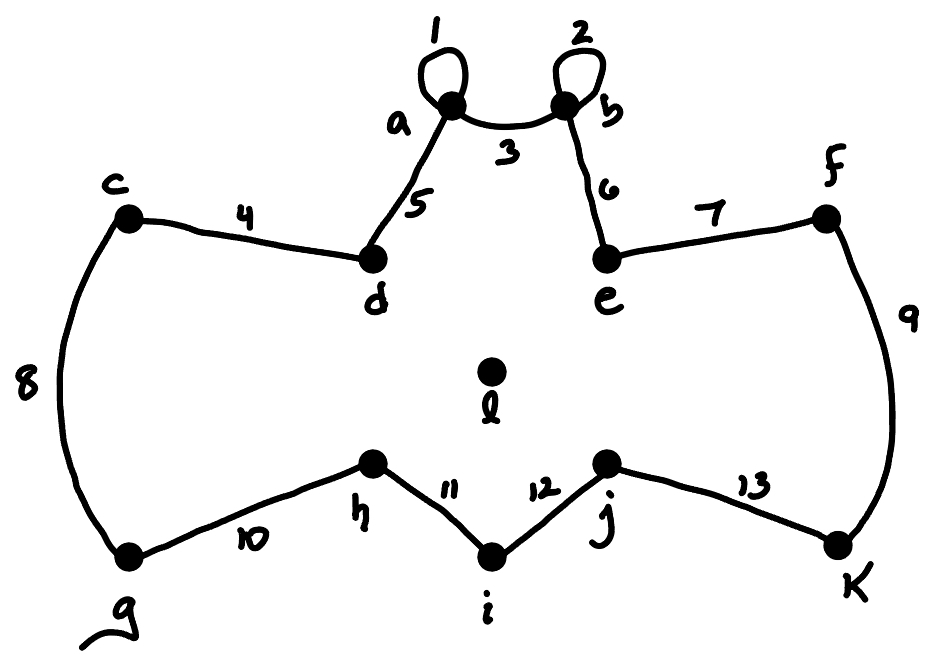
\includegraphics[width=0.45\textwidth]{graph4.jpg}
	\end{figure}

\begin{2enumerate}
\item What is $|V(G)|$?
\item What is $|E(G)|$?
\item Are there loops? Explain. 
\item Are there parallel edges? Explain. 
\item Are $7$ and $9$ adjacent? Explain. 
\item Are $h$ and $j$ adjacent? Explain. 
\item Is the graph connected? Explain. 
\item Are there isolated vertices? Explain. 
\item What is $\deg(b)$?
\item What is the degree of the graph?
\end{2enumerate}



\newpage



% Question 7
\newpage
\question[10] Showing all your work and fully justifying your reasoning, complete the following:
	\begin{enumerate}[(a)]
	\item Sketch the bipartite graph $K_{6,2}$.
	\item Is a complete graph with $n$ vertices, $K_n$, connected for all $n$? Explain. 
	\item Is every bipartite graph simple? Explain. 
	\item For $n > 2$, can $K_n$ be isomorphic to $K_{r, s}$ for some $r, s$? Explain. 
	\end{enumerate}



\newpage



% Question 8
\newpage
\question[10] A gambler is playing a dice game using a specially made six-sided die. This die has atypical probabilities. The probabilities for this die are partially given below. \par
	\begin{table}[!ht]
	\centering 
	\begin{tabular}{|c||c|c|c|c|c|c|} \hline 
	$n$ & $1$ & $2$ & $3$ & $4$ & $5$ & $6$ \\ \hline 
	$P(n)$ & $\dfrac{3\rule{0pt}{2.9ex}}{15\rule[-1.3ex]{0pt}{0pt}}$ & \phantom{$\dfrac{00}{00}$} & $\dfrac{4}{15}$ & $\dfrac{2}{15}$ & $\dfrac{3}{15}$ & $\dfrac{1}{15}$ \\ \hline 
	\end{tabular}
	\end{table} \par
If the player rolls a $1$ or $2$, they must pay \$3 or \$2, respectively. If the player rolls a $3$, they win/lose nothing. If the player rolls a $4$, $5$, or $6$, they win \$1, \$2, or \$80, respectively. 
        \begin{enumerate}[(a)]
        \item Find $P(2)$. 
        \item Find the amount that one wins `on average' playing this game, i.e. the expected value. 
        \item If one must pay \$20 upfront and then \$2 each time they wish to roll the die, should one play this game? Explain. 
        \end{enumerate}



\newpage



% Question 9
\newpage
\question[10] Let $G$ be a graph with the adjacency matrix, $A_G$, given below.
	\[
	\begin{pmatrix}
	0 & 1 & 2 & 0 & 0 & 0 & 0 & 0 & 0 & 0 \\
	1 & 0 & 0 & 1 & 0 & 0 & 0 & 0 & 0 & 0 \\
	1 & 1 & 0 & 0 & 0 & 0 & 0 & 0 & 0 & 0 \\
	1 & 0 & 1 & 1 & 0 & 0 & 0 & 0 & 0 & 0 \\
	0 & 0 & 0 & 0 & 0 & 0 & 0 & 0 & 0 & 0 \\
	0 & 0 & 0 & 0 & 0 & 2 & 0 & 1 & 0 & 0 \\
	0 & 0 & 0 & 0 & 0 & 1 & 0 & 1 & 0 & 0 \\
	0 & 0 & 0 & 0 & 0 & 2 & 0 & 0 & 0 & 0 \\
	0 & 0 & 0 & 0 & 0 & 0 & 0 & 0 & 0 & 1 \\
	0 & 0 & 0 & 0 & 0 & 0 & 0 & 0 & 1 & 0 \\
	\end{pmatrix}
	\]

\begin{enumerate}[(a)]
\item Is $G$ directed or undirected? Explain. 
\item How many vertices and edges does $G$ have? Explain. 
\item Does $G$ have isolated vertices? Explain. 
\item How many connected components does $G$ have? Explain. 
\item Does $G$ have any loops? If so, how many. If not, explain why. 
\item Find $\deg^+ v_4$ and $\deg^- v_4$. 
\end{enumerate}



\newpage



% Question 10
\newpage
\question[10] The RMS Titanic was a British passenger ship that sank on its maiden voyage across the Atlantic Ocean after striking an iceberg---killing the majority of its 2,224 passengers. A summary of the mortality statistics for the Titanic are given below. 
        \begin{table}[h]
        \centering
        \scalebox{0.87}{%
        \begin{tabular}{|c|c|c|c|c||c|} \hline
         & Men & Women & Boys & Girls & Total \\ \hline 
         Survived & 338 & 316 & 29 & 27 & 710 \\ \hline
         Died & 1352 & 109 & 35 & 18 & 1514 \\ \hline \hline
         Total & 1690 & 425 & 64 & 45 & 2224 \\ \hline
        \end{tabular}} \hfill \scalebox{0.87}{\begin{tabular}{|c||c|c||c|} \hline
        & Survived & Died & Total \\ \hline \hline
        First Class Men & 57 & 118 & 175 \\ \hline
        First Class Women & 140 & 4 & 144 \\ \hline
        First Class Children & 5 & 1 & 6 \\ \hline
        Second Class Men & 14 & 154 & 168 \\ \hline
        Second Class Women & 80 & 13 & 93 \\ \hline
        Second Class Children & 24 & 0 & 24 \\ \hline
        Third Class Men & 75 & 387 & 462 \\ \hline
        Third Class Women & 76 & 89 & 165 \\ \hline
        Third Class Children & 27 & 52 & 79 \\ \hline
        Crew (Men) & 192 & 693 & 885 \\ \hline
        Crew (Women) & 20 & 3 & 23 \\ \hline \hline
        Total & 710 & 1514 & 2224 \\ \hline
        \end{tabular}}
        \end{table}

\begin{enumerate}[(a)]
\item Find the probability that a randomly selected person aboard the Titanic survived or was a child.  
\item Find the probability that a randomly selected person aboard the Titanic was a female that survived the sinking.
\item Find the probability that a randomly selected person aboard the Titanic was a crew member.
\item Find the probability that a randomly selected person aboard the Titanic was a woman, if they survived the sinking.
\item Based on the data given, determine whether class was tied to, i.e. dependent on, survival expectancy. Explain how you came to your conclusion based on the data using probability.  
\end{enumerate}


\end{questions}
\end{document}